\documentclass{book}
\usepackage{physics}
\usepackage{graphicx}
\usepackage{caption}
\usepackage{amsmath}
\usepackage[shortlabels]{enumitem}
\usepackage{bm}
\usepackage{authblk}
\usepackage{empheq}
\usepackage{amsfonts}
\usepackage{esint}
\usepackage[makeroom]{cancel}
\usepackage{dsfont}
\usepackage{centernot}
\usepackage{mathtools}
\usepackage{bigints}
\usepackage{amsthm}
\theoremstyle{definition}
\newtheorem{defn}{Definition}[section]
\newtheorem{prop}{Proposition}[section]
\newtheorem{rmk}{Remark}[section]
\newtheorem{thm}{Theorem}[section]
\newtheorem{exmp}{Example}[section]
\newtheorem{prob}{Problem}[section]
\newtheorem{sln}{Solution}[section]
\newtheorem*{prob*}{Problem}
\newtheorem{exer}{Exercise}[section]
\newtheorem*{exer*}{Exercise}
\newtheorem*{sln*}{Solution}
\usepackage{empheq}
\usepackage{hyperref}
\usepackage{tensor}
\usepackage{xcolor}
\hypersetup{
	colorlinks,
	linkcolor={black!50!black},
	citecolor={blue!50!black},
	urlcolor={blue!80!black}
}

\usepackage{qcircuit}




\newcommand*\widefbox[1]{\fbox{\hspace{2em}#1\hspace{2em}}}

\newcommand{\p}{\partial}
\newcommand{\R}{\mathbb{R}}
\newcommand{\C}{\mathbb{C}}
\newcommand{\lag}{\mathcal{L}}
\newcommand{\nn}{\nonumber}
\newcommand{\ham}{\mathcal{H}}
\newcommand{\M}{\mathcal{M}}
\newcommand{\I}{\mathcal{I}}
\newcommand{\K}{\mathcal{K}}
\newcommand{\F}{\mathcal{F}}
\newcommand{\w}{\omega}
\newcommand{\lam}{\lambda}
\newcommand{\al}{\alpha}
\newcommand{\be}{\beta}
\newcommand{\x}{\xi}


\newcommand{\Else}{\text{else}}
\newcommand{\N}{\mathcal{N}}


\newcommand{\sig}{\bm\sigma}
\newcommand{\n}{\mathbf{n}}
\newcommand{\X}{\mathbf{X}}
\newcommand{\s}{\mathbf{S}}

\newcommand{\G}{\mathcal{G}}

\newcommand{\f}[2]{\frac{#1}{#2}}

\newcommand{\ift}{\infty}

\newcommand{\lp}{\left(}
\newcommand{\rp}{\right)}

\newcommand{\lb}{\left[}
\newcommand{\rb}{\right]}

\newcommand{\lc}{\left\{}
\newcommand{\rc}{\right\}}


\newcommand{\V}{\mathbf{V}}
\newcommand{\U}{\mathbf{U}}
\newcommand{\Id}{\mathbb{I}}
\newcommand{\D}{\mathcal{D}}
\newcommand{\Z}{\mathbf{Z}}
\newcommand{\had}{\mathbf{H}}
\newcommand{\Y}{\mathbf{Y}}
%\setcounter{chapter}{-1}


\makeatletter
\renewcommand{\@chapapp}{Part}
%\renewcommand\thechapter{$\bf{\ket{\arabic{chapter}}}$}
%\renewcommand\thesection{$\bf{\ket{\arabic{section}}}$}
%\renewcommand\thesubsection{$\bf{\ket{\arabic{subsection}}}$}
%\renewcommand\thesubsubsection{$\bf{\ket{\arabic{subsubsection}}}$}
\makeatother



\usepackage{subfig}
\usepackage{listings}
\captionsetup[lstlisting]{margin=0cm,format=hang,font=small,format=plain,labelfont={bf,up},textfont={it}}
\renewcommand*{\lstlistingname}{Code \textcolor{violet}{\textsl{Mathematica}}}
\definecolor{gris245}{RGB}{245,245,245}
\definecolor{olive}{RGB}{50,140,50}
\definecolor{brun}{RGB}{175,100,80}
\lstset{
	tabsize=4,
	frame=single,
	language=mathematica,
	basicstyle=\scriptsize\ttfamily,
	keywordstyle=\color{black},
	backgroundcolor=\color{gris245},
	commentstyle=\color{gray},
	showstringspaces=false,
	emph={
		r1,
		r2,
		epsilon,epsilon_,
		Newton,Newton_
	},emphstyle={\color{olive}},
	emph={[2]
		L,
		CouleurCourbe,
		PotentielEffectif,
		IdCourbe,
		Courbe
	},emphstyle={[2]\color{blue}},
	emph={[3]r,r_,n,n_},emphstyle={[3]\color{magenta}}
}


\begin{document}
	\begin{titlepage}\centering
		\clearpage
		\title{{\textsc{\textbf{STATISTICAL INFERENCE}}}\\ \smallskip - A Quick Guide - \\}
		\author{\bigskip Huan Q. Bui}
		\affil{Colby College\\$\,$\\ PHYSICS \& MATHEMATICS\\ Statistics \\$\,$\\Class of 2021\\}
		\date{\today}
		\maketitle
		\thispagestyle{empty}
	\end{titlepage}

\subsection*{Preface}
\addcontentsline{toc}{subsection}{Preface}

Greetings,\\

This guide is based on SC482: Statistical Inference, taught by Professor Liam O'Brien. The guide consists of lecture notes and material from \textit{Introduction to Mathematical Statistics, 8th edition} by Hogg, McKean, and Craig. A majority of the text will be reading notes and solutions to selected problems. \\

As this is intended only to be a reference source, I might not be as meticulous with my explanations as I have been in some other guides. \\

Enjoy! 

\newpage
\tableofcontents
\newpage




\chapter{Special Distributions}
\newpage


\section{The Binomial and Related Distributions}
If we let the random variable $X$ equal the number of observed successes in $n$ independent Bernoulli trials, each with success probability of $p$, then $X$ follows the binomial distribution.s\\



A binomial pmf is given by
\begin{align}
\boxed{p(x) = \begin{cases}
{n\choose x}p^x(1-p)^{n-x} \quad x=0,1,2,\dots \\
0, \quad \text{else}
\end{cases}}
\end{align}
Using the binomial expansion formula, we can easily check that
\begin{align}
\boxed{\sum_x p(x) = 1}
\end{align}
The mgf of a binomial distribution is obtained by:
\begin{align}
\boxed{M_{\text{bin}}(t) = E[e^{tx}] = \sum_x e^{tx}p(x) = \lb (1-p) + pe^t \rb^n \forall t \in \R}
\end{align}
With this, we can find the mean and variance for $p(x)$:
\begin{align}
\boxed{\mu = M'(0) = n, \quad \sigma^2 = M''(0) = np(1-p)}
\end{align}

\noindent \textbf{Theorem:} Let $X_1, X_2, \dots, X_m$ be independent binomial random variables such that $X_i \sim \text{bin}(n_i, p), i = 1,2,\dots,m$. Then 
\begin{align}
\boxed{Y = \sum^m_{i=1} X_i \sim \text{bin}\lp \sum^m_{i=1}n_i, p \rp}
\end{align}
\noindent \textit{Proof:} We prove this via the mgf for $Y$. By independence, we have that
\begin{align}
M_Y(t) = \prod^m_{i=1}(1-p + pe^t)^{n_i} = (1-p + pe^t)^{\sum^m_{i=1} n_i}
\end{align}
The mgf completely determines the distribution which $Y$ follows, so we're done. \qed



\subsection{Negative Binomial \& Geometric Distribution}
Consider a sequence of independent Bernoulli trials with constant probability $p$ of success. The random variable $Y$ which denotes the total number of failures in this sequence before the $r$th success follows the negative binomial distribution.\\


A negative binomial pmf is given by
\begin{align}
\boxed{p_Y(t) = \begin{cases}
{(y+r-1)\choose{r-1}}p^r(1-p)^y \quad y = 0,1,2,\dots\\
0, \quad \text{else}
\end{cases}}
\end{align} 
The mgf of this distribution is 
\begin{align}
\boxed{M(t) = p^r[1-(1-p)e^{t}]^{-r}}
\end{align}
 
 
When $r=1$, $Y$ follows the geometric distribution, whose pmf is given by
\begin{align}
\boxed{p_Y(y) = p(1-p)^y,\quad y = 0,1,2,\dots}
\end{align}
The mgf of this distribution is 
\begin{align}
\boxed{M(t) = p[1-(1-p)e^{t}]^{-1}}
\end{align}




\section{Multinomial Distribution}
We won't worry about this for now.
\section{Hypergeometric Distribution}
We won't worry about this for now.



\section{The Poisson Distribution}

The Poisson distribution gives the probability of observing $x$ occurrences of some rare events characterized by rate $\lambda > 0$. The pmf is given by
\begin{align}
\boxed{p(x) = \begin{cases}
	\f{\lambda^x e^{-\lambda}}{x!}, \quad x = 0,1,2,\dots\\
	0, \quad \text{else}
	\end{cases}}
\end{align}
We say a random parameter with the pmf of the form of $p(x)$ follows the Poisson distribution with parameter $\lambda$.  \\

The mgf of a Poisson distribution is given by 
\begin{align}
\boxed{M(t)= e^{-\lambda (e^t-1)}}
\end{align}
From here, we can find the mean and variance:
\begin{align}
\boxed{\mu = M'(0) = \lambda, \quad \sigma^2 = M''(0) = \lambda}
\end{align}


\noindent\textbf{Theorem:} If $X_1, \dots, X_n$ are independent random variables, each $X_i \sim \text{Poi}(\lambda_i)$, then 
\begin{align}
\boxed{Y = \sum^n_{i=1} X_i \sim \text{Poi}\lp \sum^n_{i=1}\lambda_i \rp}
\end{align}
\noindent \textit{Proof:} We once again prove this via the mgf of $Y$:
\begin{align}
M_Y(t) = \prod^n_{i=1}e^{\lambda_i (e^t-1)} = e^{\sum^n_{i=1} \lambda_i(e^t - 1)}
\end{align}
\qed



\section{The $\Gamma, \chi^2, \beta$ distributions}

The gamma function of $\alpha > 0$ is given by
\begin{align}
\Gamma(\alpha) =\int^\infty_0 y^{\alpha-1}e^{-y}\,dy,
\end{align}
which gives $\Gamma(1) = 1$ and $\Gamma(\alpha) = (\alpha-1)\Gamma(\alpha-1)$. 

\subsection{The $\Gamma$ and exponential distribution}
A continuous random variable $X \sim \Gamma(\alpha,\beta)$ where $\alpha > 0$ and $\beta > 0$ whenever its pdf is
\begin{align}
\boxed{f(x) = \begin{cases}
	\f{1}{\Gamma(\alpha)\beta^\alpha}x^{\alpha-1} e^{-x/\beta}, \quad 0 < x < \infty\\
	0, \quad \text{else}
	\end{cases}}
\end{align}
The mgf for $X$ is obtained via the change of variable $y = x(1-\beta t)/\beta$, where $t < 1/\beta$:
\begin{align}
\boxed{M(t) = \int^\infty_0 \f{1}{\Gamma(\alpha)\beta^\alpha} x^{\alpha-1} e^{-x(1-\beta t)/\beta}\,dx = \f{1}{(1-\beta t)^\alpha}}
\end{align}
From here, we can find the mean and variance:
\begin{align}
\boxed{\mu = M'(0) = \alpha\beta, \quad \sigma^2 = \alpha \beta^2}
\end{align}

The $\Gamma(1,\beta)$ distribution is a special case, and it is called the \textbf{exponential distribution} with parameter $1/\beta$.\\

\noindent\textbf{Theorem:} Let $X_1, \dots, X_n$ be independent random variables, with $X_i \sim \Gamma(\alpha_i, \beta)$. Then
\begin{align}
\boxed{Y = \sum^n_{i=1} X_i \sim \Gamma\lp \sum^n_{i=1}\alpha_i, \beta \rp}
\end{align} 
\noindent\textit{Proof:} Can you guess via which device we prove the statement above?\qed


\subsection{The $\chi^2$ distribution}

The $\chi^2$ distribution is a special case of the gamma distribution where $\alpha = r/2, r \in \mathbb{N}^*$ and $\beta = 2$. If a continuous r.v. $X \sim \chi^2(r)$ then its pdf is 
\begin{align}
\boxed{f(x) = \begin{cases}
\f{1}{\Gamma(r/2)2^{r/2}} x^{r/2-1}e^{-x/2}, \quad 0 < x < \infty\\
0, \quad \text{else}
\end{cases}}
\end{align}
Its mgf is 
\begin{align}
\boxed{M(t) = (1-2t)^{-r/2}, \quad t < \f{1}{2}}
\end{align}

\noindent\textbf{Theorem:} Let $X \sim \chi^2(r)$ and $k > -r/2$ be given. Then $ E[X^k] $ exists and is given by
\begin{align}
\boxed{E[X^k] = \f{2^k\Gamma\lp r/2 + k \rp}{\Gamma(r/2)}}
\end{align}
\noindent \textit{Proof:} is proof is purey computational and is left to the reader. \qed\\

From here, we note that all moments of the $\chi^2$ distribution exist.\\

\noindent\textbf{Theorem:} Let $X_1, \dots, X_n$ be r.v. with $X_i \sim \chi^2(r_i)$. Then
\begin{align}
\boxed{Y = \sum^n_{i=1}X_i \sim \chi^2\lp \sum^n_{i=1}r_i \rp}
\end{align}
\noindent \textit{Proof:} we once again find the mgf for $Y$. \qed\\


\subsection{The $\beta$ distribution}

The $\beta$ distribution differs from the other continuous ones we've discussed so far because its support are bounded intervals. \\

I will skip most of the details here, except mentioning that we can derive the beta distribution from the a pair of independent $\Gamma$ random variables. Suppose $Y = X_1/(X_1 + X_2)$ where $X_i \sim \Gamma(\alpha, \beta)$ then the pdf of $Y$ is that of the beta distribution:
\begin{align}
\boxed{g(y) = \begin{cases}
	\f{\Gamma(\alpha+\beta)}{\Gamma(\alpha)\Gamma(\beta)}y^{\alpha-1}(1-y)^{\beta-1},\quad 0< y< 1\\
	0,\quad \text{else}
	\end{cases}}
\end{align} 
The mean and variance of $Y$ are
\begin{align}
\boxed{\mu = \f{\alpha}{\alpha+ \beta}, \quad \sigma^2 = \f{\alpha\beta}{(\al + \be + 1)(\al + \be)^2}}
\end{align}





\section{The Normal distribution}

I have dedicated a large chunk in the \href{https://huanqbui.com/LaTeX projects/HuanBui_QM/HuanBui_QM.pdf}{\underline{QFT}} notes to evaluating Gaussian integrals, so I won't go into that here. \\

$X \sim \mathcal{N}(\mu,\sigma^2)$ whenever its pdf is
\begin{align}
\boxed{f(x) = \f{1}{\sqrt{2\pi \sigma^2}} \exp\lp -\f{1}{2}\f{(x-\mu)^2}{\sigma^2} \rp, \quad -\infty < x < \infty}
\end{align}
where $\mu$ and $\sigma^2$ are the mean and variance of $X$, respectively. \\

The mgf of $X$ is can be obtained via the substitution $X = \sigma Z + \mu$:
\begin{align}
\boxed{M(t) = \exp\lp \mu t  + \f{1}{2}\sigma^2 t^2 \rp}
\end{align}
We note the following correspondence for $X = \sigma Z + \mu$:
\begin{align}
X \sim \mathcal{N}(\mu,\sigma^2) \iff {Z \sim \mathcal{N}(0,1)}
\end{align}

\noindent\textbf{Theorem:} $X \sim \mathcal{N}(\mu, \sigma^2) \implies V = (X-\mu)^2/\sigma^2 \sim \chi^2(1)$, i.e. a standardized, squared normal follows a chi-square distribution. \\

\noindent \textit{Proof:} The proof isn't too hard. Let us write $V$ as $W^2$ and so $W \sim \mathcal{N}(0,1)$.  We consider the cdf $G(v)$ for $V$, with $v \geq 0$:
\begin{align}
G(v) = P( W^2 \leq v) = P( -\sqrt{v} \leq  W  \leq \sqrt{v} ) = 2\int^{\sqrt{v}}_0 \f{1}{ \sqrt{2\pi} } e^{-w^2/2}\,dw
\end{align}
with $G(v) = 0$ whenever $v<0$. From here, we can see that the pdf for $v$, under the change of notation $w \to \sqrt{y}$, is
\begin{align}
g(v) = G'(v) = \f{d}{dv}\lc \int^v_0 \f{1}{\sqrt{2\pi}\sqrt{y}}e^{-y/2}\,dy \rc, \quad 0 \geq v
\end{align}
or $0$ otherwise. This means
\begin{align}
\boxed{g(v) = \begin{cases}
\f{1}{\sqrt{\pi}\sqrt{2}} v^{1/2-1}e^{-v/2}, \quad 0 < v< \infty\\
0, \quad \text{else}
\end{cases}}
\end{align}
Using the fact that $\Gamma(1/2) = \sqrt{\pi}$ and by verifying that $g(v)$ integrates to unity we show $V \sim \chi^2(1)$. \qed\\



\noindent\textbf{Theorem:}  Let $X_1, \dots, X_n$ be independent r.v. with $X_i \sim \mathcal{N}(\mu_i, \sigma_i^2)$. Then for constants $a_1,\dots, a_n$
\begin{align}
\boxed{Y = \sum^n_{i=1}a_i X_i \sim \mathcal{N}\lp \sum^n_{i=1}a_i\mu_i, \sum^n_{i=1}a_i^2\sigma^2_i \rp}
\end{align}
\noindent \textit{Proof:} We once again prove this kind of theorems via the mgf for $Y$:
\begin{align}
M(t) &= \prod^n_{i=1}\exp\lp ta_i\mu_i + \f{1}{2}a_i^2\sigma_i^2 \rp \nn\\
&= \exp\lc t\sum^n_{i=1}a_i\mu_i + \f{1}{2}t^2\sum^n_{i=1}a_i^2\sigma_i^2 \rc
\end{align}
which is the mgf for the normal with the corresponding mean and variance above. \qed\\


\textbf{Corollary:} Let $X_1, \dots, X_n \sim \mathcal{N}(\mu,\sigma^2)$. Then 
\begin{align}
\boxed{\bar{X} = \f{\sum^n_{i=1} X_i}{n} \sim \mathcal{N}\lp \mu, \sigma^2/n \rp}
\end{align} 
\noindent \textit{Proof:} the proof is left to the reader.



\subsection{Contaminated Normal}

We won't worry about this for now.


\section{The Multivariate Normal}
I'll just jump straight to the $n$-dimensional generalization. Evaluations of high-dimensional Gaussian integrals and moments can also be found in the \href{https://huanqbui.com/LaTeX projects/HuanBui_QM/HuanBui_QM.pdf}{\underline{QFT}} notes. \\

We say an $n$-dimensional random vector $\X$ has a multivariate normal distribution if its mgf is 
\begin{align}
\boxed{M_{\X}(t) = \exp\lp \mathbf{t}^\top\bm{\mu} + \f{1}{2}\mathbf{t}^\top\mathbf{\Sigma}\mathbf{t} \rp}
\end{align}
for all $\mathbf{t} \in \R^n$, where $\mathbf{\Sigma}$ is a symmetric, positive semi-definite matrix and $\bm{\mu} \in \R^n$. For short, we say $\X \sim \mathcal{N}_n(\bm{\mu}, \mathbf{\Sigma})$.   \\

\noindent\textbf{Theorem:} Suppose $\X \sim \mathcal{N}_n(\bm{\mu}, \mathbf{\Sigma})$ where $\mathbf{\Sigma}$ is positive definite. Then 
\begin{align}
\boxed{\Y = (\X - \bm{\mu})^\top \mathbf{\Sigma}^{-1}(\X - \bm{\mu}) \sim\chi^2(1)}
\end{align}

\noindent\textbf{Theorem:} If $\X \sim \mathcal{N}_n(\bm{\mu},\mathbf{\Sigma})$ then
\begin{align}
\boxed{\Y = \mathbf{A}\X + \mathbf{b} \sim \mathcal{N}_n(\mathbf{A}\bm{\mu} + \mathbf{b})}
\end{align}
\noindent \textit{Proof:} The proof once again uses the mgf for $\Y$, but also some linear algebra manipulations. \qed\\

There are many other theorems and results related to this topic, but I won't go into them for now. \\




\section{The $t$- and $F$-distributions}


These two distributions are useful in certain problems in statistical inference. 

\subsection{The $t$-distribution}
Suppose $W \sim \mathcal{N}(0,1)$ and $V \sim \chi^2(r)$ and that they are independent. Then the joint pdf of $W$ and $V$, called $h(w,v)$, is the product of the pdf's of $W$ and $V$:
\begin{align}
h(w,v) = \begin{cases}
\f{1}{\sqrt{2\pi}}e^{-w^2/2}\f{1}{\Gamma(r/2)2^{r/2}}v^{r/2-1}e^{-v/2}, \quad w\in \R, v >0\\
0, \quad \Else
\end{cases}
\end{align}
Now we define a new variable $T = W/\sqrt{V/r}$ and consider the transformation:
\begin{align}
t = \f{w}{\sqrt{v/r}} \quad u=v
\end{align}
which bijectively maps the parameter space $(w,v) = \R\times \R^+$ to $(t,u)=\R \times \R^+$. The absolute value of the Jacobian of the transformation is given by
\begin{align}
\abs{J} = \abs{\det\begin{pmatrix}
	\p_tw & \p_u w\\
	\p_tv & \p_u v
	\end{pmatrix}} = \f{\sqrt{u}}{\sqrt{r}}.
\end{align} 
With this, the joint pdf of $T$ and $U \equiv V$ is given by
\begin{align}
g(t,u) =  \abs{J}h\lp \f{t\sqrt{u}}{\sqrt{r}},u \rp
= \begin{cases}
\f{u^{r/2-1}}{\sqrt{2\pi} \Gamma(r/2) 2^{r/2}}\exp\lb -\f{u}{2} \lp 1 + \f{t^2}{r} \rp \rb \f{\sqrt{u}}{\sqrt{r}}, \quad t\in \R, u \in \R^+\\
0,\quad \Else
\end{cases}
\end{align}
By integrating out $u$ we obtain the marginal pdf for $T$:
\begin{align}
g_1(t) &= \int^\infty_{-\infty}g(t,u)\,du \nn\\
&= \int^\infty_0 \f{u^{(r+1)/2-1}}{\sqrt{2\pi r} \Gamma(r/2) 2^{r/2}}\exp\lb -\f{u}{2} \lp 1 + \f{t^2}{r} \rp \rb \,du.
\end{align}
Via the substitution $z = u[1 + (t^2/r)]/2$ we can evaluate the integral to find for $t\in \R$
\begin{align}
\boxed{g_1(t) = \f{\Gamma[(r+1)/2]}{\sqrt{\pi r}\Gamma(r/2)}  \f{1}{(1 + t^2/r)^{(r+1/2)}} }
\end{align}

A r.v. $T$ with this pdf is said to follow the $t$-distribution (or the Student's $t$-distribution) with $r$ degrees of freedom. The $t$-distribution is symmetric about 0 and has a unique maximum at 0. As $r\in \infty$, the $t$-distribution converges to $\N(0,1)$. \\

The mean of $T \sim \text{Stu}(r)$ is zero. The variance can be found to be $\text{Var}(T) = E[T^2] = \f{r}{r-2}$, so long as $r>2$. 
   





\subsection{The $F$-distribution}
Let $U \sim \chi^2(r-1), V\sim \chi^2(r_2)$ be given. Then the joint pdf of $U$ and $V$ is once again the product of their pdf's:
\begin{align}
h(u,v) = \begin{cases}
\f{1}{\Gamma(r_1/2)\Gamma(r_2/2) 2^{(r_1+r_2)/2}}u^{r_1/2-1}v^{r_2/2-1}e^{-(u+v)/2}, \quad u,v \in \R^+\\
0,\quad \Else
\end{cases}
\end{align}
Define the new random variable 
\begin{align}
W = \f{U/r_1}{V/r_2}
\end{align}
whose pdf $g_1(w)$ we are interested in finding. Consider the transformation
\begin{align}
w = \f{u/r_1}{v/r_2}, \quad z=v
\end{align}
which bijectively maps $(u,v) = \R^+\times \R^+ \to (w,z) = [\R^+\times \R^+]$. Like last time, the absolute value of the Jacobian can be found to be
\begin{align}
\abs{J} = \f{r_1}{r_2}z.
\end{align}
The joint pdf $g(w,z)$ of the random variables $W$ and $Z=V$ is obtained from by scaling $h(u,v)$ by $\abs{J}$ and applying the variable transformation:
\begin{align}
g(w,z) = 
\f{1}{\Gamma(r_1/2)\Gamma(r_2/2) 2^{\f{r_1+r_2}{2}}} \lp \f{r_1 zw}{r_2} \rp^{\f{r_1-2}{2}}z^{\f{r_2-2}{2}}\exp\lb -\f{z}{2}\lp \f{r_1w}{r_2} +1 \rp\rb \f{r_1z}{r_2}
\end{align}
so long as $(w,z)\in \R^+\times \R^+$ and 0 otherwise. We then proceed to find the marginal pdf $g_1(w)$ of $W$ by integrating out $z$. By considering the change of variables:
\begin{align}
y = \f{z}{2}\lp \f{r_1w}{r_2} + 1 \rp
\end{align}
we can evaluate the integral and find the marginal pdf of $W$ to be 
\begin{align}
g_1(w) = \begin{cases}
\f{\Gamma[(r_1+r_2)/2](r_1/r_2)^{r_1/2}}{\Gamma(r_1/2)\Gamma(r_2/2)}\f{w^{r_1/2-1}}{(1+r_1w/r_2)^{(r_1+r_2)/2}}, \quad w\in \R^+\\
0, \quad \Else
\end{cases}
\end{align}
$W$, which is the ratio of two independent chi-quare variables $U,V$, is said to follow an $F$-distribution with degrees of freedom $r_1$ and $r_2$. We call the ratio $W = (U/r_1)/(V/r_2)$ the ``$F$'' ratio. \\

The mean of $W$ is $E[F] = \f{r_2}{r_2-2}$. When $r_2$ is large, $E[F] \to 1$.  


\subsection{The Student's Theorem}

Here we will create the connection between the normal distribution and the $t$-distribution. This is an important result for the later topics on inference for normal random variables. \\

\noindent\textbf{Theorem:} Let $X_1, \dots, X_n$ be iid r.v. with $X_i \sim \N(\mu,\sigma^2) \forall i$. Define the r.v.'s
\begin{align}
\bar{X} &= \f{1}{n}\sum^n_{i=1}X_i\\
S^2 &= \f{1}{n-1}\sum^n_{i=1}(X_i - \bar{X})^2.
\end{align}
Then
\begin{enumerate}[(a)]
	\item $\bar{X} \sim \N(\mu, \sigma^2/n)$.
	\item $\bar{X}$ and $S^2$ are independent. 
	\item $(n-1)S^2/\sigma^2 \sim \chi^2(n-1)$.
	\item The variable $\bar{T} = (\bar{X} - \mu)/(S/\sqrt{n})$ follows the Student's $t$-distribution with $n-1$ degrees of freedom. 
	\begin{align}
	\bar{T} = \f{\bar{X} - \mu}{S/\sqrt{n}} \sim \text{Stu}(n-1).
	\end{align}
\end{enumerate}

\noindent \textit{Proof:} The proof is good, so I will reproduce it here. Because $X_i \sim \N(\mu,\sigma^2) \forall i$, $\X \sim \N_n\lp \mu \mathbf{1}, \sigma^2\mathbf{1} \rp$, where $\mathbf{1}$ denotes the $n$-vector whose components are all 1. Now, consider $\mathbf{v}^\top = (1/n)\mathbf{1}^\top$. We see that $\bar{X} = \mathbf{v}^\top \X$. Define the random vector $\Y = (X_1 - \bar{X}, \dots, X_2 - \bar{X})^\top$ and consider the (true) equality:
\begin{align}
\mathbf{W} = \begin{pmatrix}
\bar{X} \\ \Y
\end{pmatrix} = \underbrace{\begin{pmatrix}
\mathbf{v}^\top \\ 
\Id - \mathbf{1}\mathbf{v}^\top
\end{pmatrix}}_{\text{the transformation}} \X
\end{align} 
which just restates our definitions nicely. We see that $\mathbf{W}$ is a result of a linear transformation of multivariate normal random vector, and so it follows that $\mathbf{W} \sim \N_{n+1}$ with mean 
\begin{align}
E[\mathbf{W}] = \begin{pmatrix}
\mathbf{v}^\top \\
\Id - \mathbf{1}\mathbf{v}^\top
\end{pmatrix}\mu \mathbf{1} = \begin{pmatrix}
\mu \\ \mathbf{0}_n
\end{pmatrix}
\end{align}
and the covariance matrix
\begin{align}
\mathbf{\Sigma} = \begin{pmatrix}
\mathbf{v}^\top \\
\Id - \mathbf{1}\mathbf{v}^\top
\end{pmatrix}\sigma^2 \Id
\begin{pmatrix}
\mathbf{v}^\top \\
\Id - \mathbf{1}\mathbf{v}^\top
\end{pmatrix}^\top = \sigma^2 \begin{pmatrix}
\f{1}{n} & \mathbf{0}_n^\top \\
\mathbf{0}_n & \Id - \mathbf{1}\mathbf{v}^\top
\end{pmatrix}
\end{align}

From here, part (a) is proven. Next, observe that $\mathbf{\Sigma}$ is diagonal, and so all covariances are zero. This means $\bar{X}$ is independent of $\mathbf{Y}$. But because $S^2 = (n-1)^{-1}\Y^\top \Y$, $\bar{X}$ is independent of $S^2$ as well. So, (b) is proven. \\

Now, consider the r.v. 
\begin{align}
V = \sum^n_{i=1} \lp\f{X_i - \mu}{\sigma}\rp^2
\end{align} 
Each summand of $V$ is a square of an $\N(0,1)$ r.v., and so each follows a $\chi^2(1)$. Because $V$ is a sum of squares of $n$ such $\chi^2(1)$'s, $V \sim\chi^2(n)$. Next, we can rewrite $V$ as
\begin{align}
V = \sum^n_{i=1}\lp \f{(X_i - \bar{X}) + (\bar{X} - \mu)}{\sigma} \rp^2 = \f{(n-1)S^2}{\sigma^2} + \lp \f{\bar{X} - \mu}{\sigma/\sqrt{n}} \rp^2.
\end{align}
By (b), the summands in the last equation is are independent. The second term is a square of a $\N(0,1)$, so it follows a $\chi^2(1)$. Taking mgfs of both sides, we get
\begin{align}
(1-2t)^{-n/2} = \underbrace{E[\exp{t(n-1)S^2/\sigma^2}]}_{M_{\text{(c)}}} (1-2t)^{-1/2}.
\end{align}
Solving for the mgf of $(n-1)S^2/\sigma^2$ we get part $(c)$. Finally, writing $T$ as
\begin{align}
T = \f{(\bar{X} - \mu)/(\sigma/\sqrt{n})}{\sqrt{(n-1)S^2/(\sigma^2(n-1))}}
\end{align}
and using (a)-(c) gives us (d). \textit{Hint}: consider what distributions the numerator and denominator of $T$ follow. \qed









\newpage
 
\section{Problems}

\noindent \textbf{3.6.4}
\begin{enumerate}[(a)]
	\item $X$ has a standard normal distribution:
	\begin{lstlisting}
	x=seq(-6,6,.01); plot(dnorm(x)~x)
	\end{lstlisting}
	\item $X$ has a $t$-distribution with 1 degree of freedom.
	\begin{lstlisting}
	lines(dt(x,1)~x,lty=2)
	\end{lstlisting}
	\item $X$ has a $t$-distribution with 3 degrees of freedom.
	\begin{lstlisting}
	lines(dt(x,3)~x,lty=2)
	\end{lstlisting}
	\item $X$ has a $t$-distribution with 10 degrees of freedom.
	\begin{lstlisting}
	lines(dt(x,10)~x,lty=2)
	\end{lstlisting}
	\item $X$ has a $t$-distribution with 30 degrees of freedom.
	\begin{lstlisting}
	lines(dt(x,30)~x,lty=2)
	\end{lstlisting}
\end{enumerate}

\begin{figure}[!htb]
	\centering
	\subfloat[]{{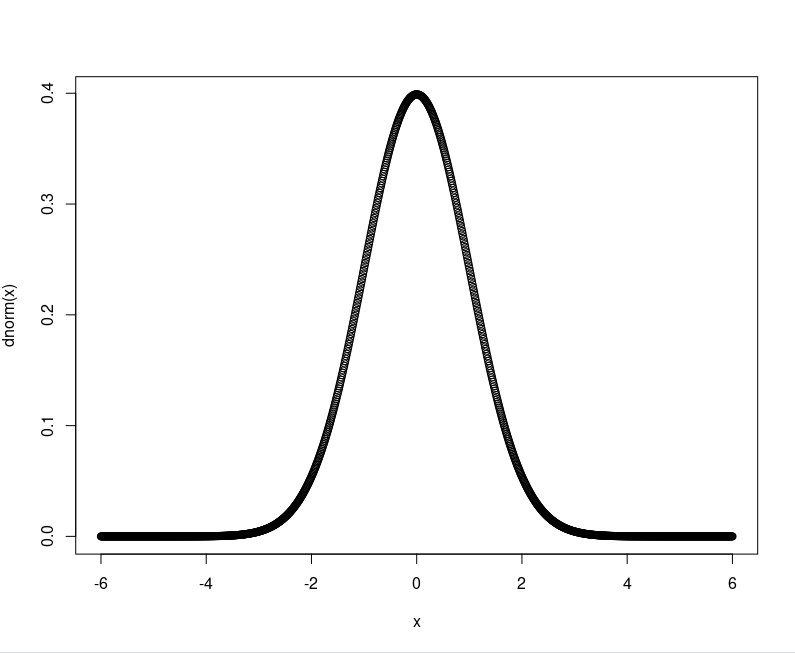
\includegraphics[width=3.35cm]{364a} }}
	\qquad
	\subfloat[]{{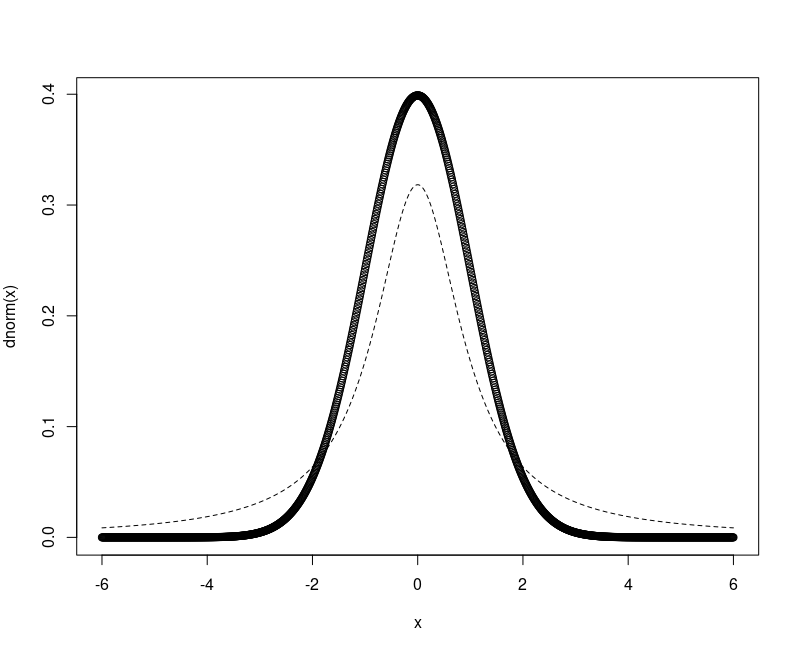
\includegraphics[width=3.35cm]{364b} }}
	\qquad
	\subfloat[]{{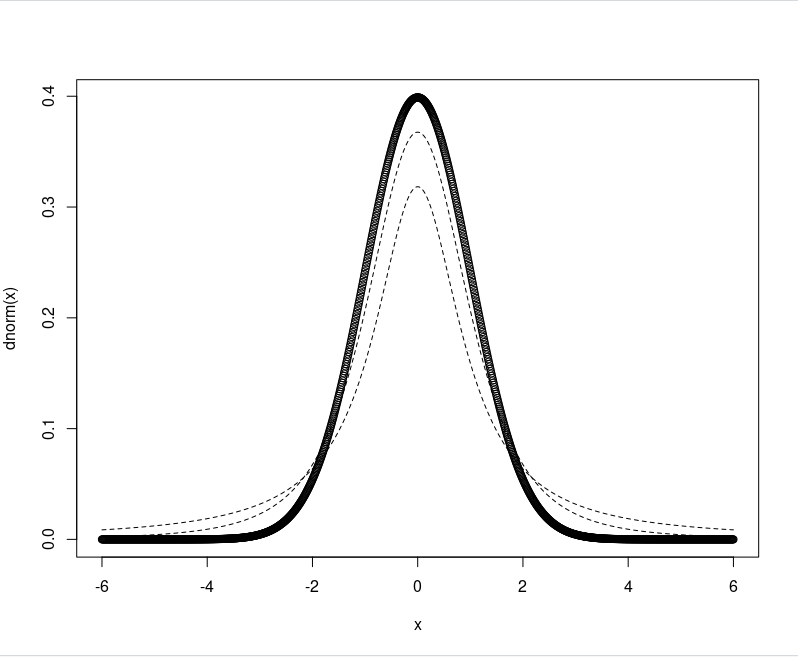
\includegraphics[width=3.35cm]{364c} }}\\
	\subfloat[]{{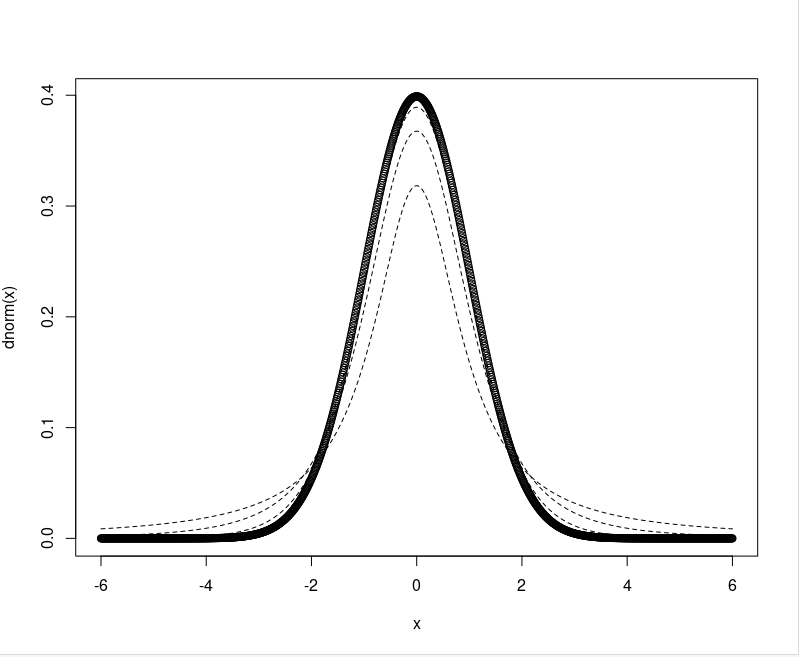
\includegraphics[width=4cm]{364d} }}
	\quad
	\subfloat[]{{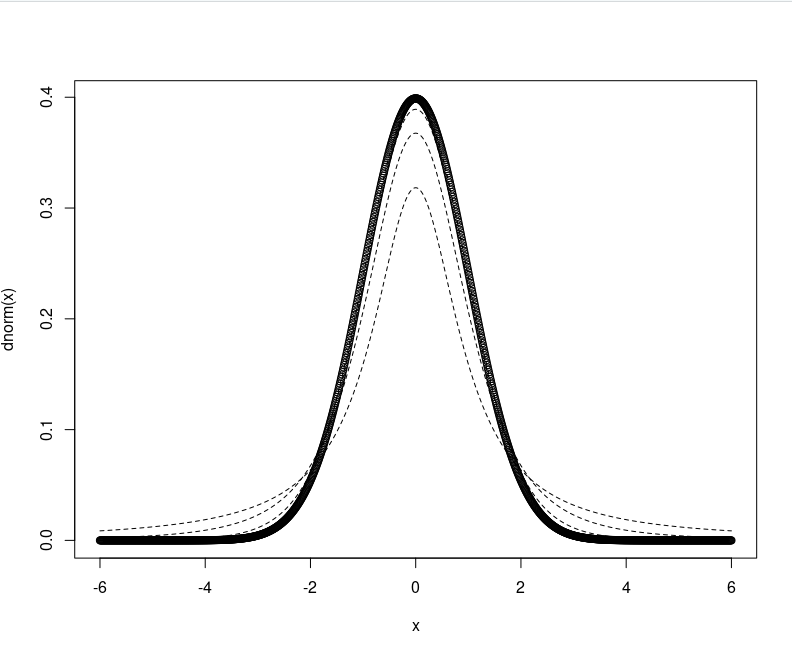
\includegraphics[width=4cm]{364e} }}
\end{figure}




\newpage
\noindent\textbf{3.6.5}
\begin{enumerate}[(a)] 
	\item $P(\abs{X} \geq 2) = 2\times[1 - P(X \leq 2)] = \textbf{0.046}$.
	\begin{lstlisting}
	> 2*(1 - pnorm(2))
	[1] 0.04550026
	\end{lstlisting}
	
	\item $P(\abs{X} \geq 2) = 2\times[1 - P(X \leq 2)] = \textbf{0.295}$.
	\begin{lstlisting}
	> 2*(1 - pt(2,1))
	[1] 0.2951672
	\end{lstlisting}
	
	\item $P(\abs{X} \geq 2) = 2\times[1 - P(X \leq 2)] = \textbf{0.139}$.
	\begin{lstlisting}
	> 2*(1 - pt(2,3))
	[1] 0.139326
	\end{lstlisting}
	
	\item $P(\abs{X} \geq 2) = 2\times[1 - P(X \leq 2)] = \textbf{0.073}$.
	\begin{lstlisting}
	> 2*(1 - pt(2,10))
	[1] 0.07338803
	\end{lstlisting}
	
	\item $P(\abs{X} \geq 2) = 2\times[1 - P(X \leq 2)] = \textbf{0.055}$.
	\begin{lstlisting}
	> 2*(1 - pt(2,30))
	[1] 0.05462504
	\end{lstlisting}
\end{enumerate}






\newpage
\noindent\textbf{3.6.11:} Let $T = W/\sqrt{V/r}$, where the independent variables $W \sim \mathcal{N}(0,1)$ and $V \sim \chi^2(r)$. Show that $T^2\sim F(r_1 = 1, r_2 = r)$. \textit{Hint}: What is the distribution of the numerator of $T^2$?\\

\noindent \textit{Solution:} Let the independent random variables $U,V$ be given, with $W\sim \N(0,1)$ and $U\sim \chi^2(r)$. The random variable $T^2$, where $T = W / \sqrt{V/r}$ is given by
\begin{align}
T^2 = \lp \f{W}{\sqrt{V/r}} \rp^2 = \f{W^2}{V/r}.
\end{align}
Because $W \sim \N(0,1)$, we have that $W^2 \sim \chi^2(1)$ (by theorem). Now, $T^2$ has the form 
\begin{align}
T^2 = \f{W^2}{V/r} = \f{W^2/1}{V/r}
\end{align}
where $1$ is the df of $\chi^2(1)$ which $W$ follows, and $r$ is the df of $\chi^2(r)$ which $U$ follows. Thus, $T^2 \sim F(1,r)$, by the definition of the $F$-distribution. \qed






\newpage

\noindent\textbf{3.6.15:} Let $X_1$, $X_2$ be iid with common distribution having the pdf 
\begin{align}
f(x) = \begin{cases}
e^{-x}, \quad 0< x < \infty\\
0, \quad \text{else}
\end{cases}
\end{align}
Show that $Z = X_1/X_2$ has an $F$-distribution.\\

\noindent \textit{Solution:}  It suffices to show that $Z$ can be written as a ratio of two $\chi^2$-distributed independent random variables. To this end, we can consider the mgf $M_X(t)$ of $X_1$, which is also identically that of $X_2$ since $X_1, X_2$ are iid:
\begin{align}
M_X(t) = E[e^{tx}] = \int^\infty_0 e^{tx}e^{-x} \,dx = (1-t)^{-1}.
\end{align}
However, this does not quite match the mgf for a $\chi^2(2)$. To circumvent this problem, we rewrite
\begin{align}
Z = \f{X_1}{X_2} =\f{2X_1/2}{2X_2/2}  = \f{(X_1+X_1)/2}{(X_2+X_2)/2},
\end{align}
as we expect $r=2$. Let $Y_1 = X_1 + X_1$. Then we have trivially $Y_1 =2X_1$, and so $\abs{J} = 2$. With this, $Y_1$ has the pdf 
\begin{align}
\tilde{f}_Y(y) = \abs{J}f(x) = 2f(x) = \begin{cases}
2e^{-y/2}, \quad 0 < y < \infty\\
0, \quad \Else
\end{cases}. 
\end{align}
From here, we find the mgf of $Y_1$ to be 
\begin{align}
M_{Y_1}(t) = E[e^{ty}] = \f{1}{2}\int^\infty_{0}e^{ty}e^{-y/2}\,dy = (1-2t)^{-1} = (1-2t)^{-2/2}, t < \f{1}{2}.
\end{align}
By symmetry, $M_{Y_2}(t)$ is identically $M_{Y_1}(t)$, and both are the mgf for $\chi^2(r=2)$. Because each mgf uniquely determines a pdf, $Y_1, Y_2 \sim \chi^2(r=2)$ identically and independently (for each depends exclusively on $X_1$, $X_2$, respectively). Therefore, 
\begin{align}
Z = \f{(X_1+X_1)/2}{(X_2+X_2)/2} = \f{Y_1/2}{Y_2/2}
\end{align}
follows the $F$-distribution with degrees of freedom $r_1 = r_2 = 2$, by definition. \qed






\newpage
\noindent\textbf{3.6.16:} Let $X_1, X_2, X_3$ be independent r.v. with $X_i \sim \chi^2(r_i)$. 
\begin{enumerate}[(a)]
	\item Show that $Y_1 = X_1/X_2$ and $Y_2 = X_1 + X_2$ are independent and that $Y_2 \sim \chi^2(r_1 + r_2)$. 
	
	\item Deduce that 
	\begin{align}
	\f{X_1/r_1}{X_2/r_2} \text{ and } \f{X_3/r_3}{(X_1 + X_2)/(r_1 + r_2)}
	\end{align}
	are independent $F$-variables. 
\end{enumerate}

\noindent \textit{Solution:}  

\begin{enumerate}[(a)]
	\item We consider the transformation
	\begin{align}
	y_1 &= u(x_1,x_2) = \f{x_1}{x_2}\\
	y_2 &= v(x_1,x_2) = x_1 + x_2.
	\end{align}
	whose inverse is 
	\begin{align}
	x_1 = \bar{u}(y_1, y_2) = \f{y_1y_2}{1+y_1}\nn\\
	x_2 = \bar{v}(y_1, y_2) = \f{y_2}{1+y_1}.
	\end{align}
	The absolute value of the Jacobian is 
	\begin{align}
	\abs{J} = \abs{\det\begin{pmatrix}
		\p_{y_1}\bar{u} & \p_{y_2}\bar{u}\\
		\p_{y_1}\bar{v} & \p_{y_2}\bar{v}\\
		\end{pmatrix}} = \f{y_2}{(1+y_1)^2},
	\end{align}
	which maps one-to-one from the space of $X_1,X_2$ $\R^+\times \R^+$ onto the space of $Y_1, Y_2$ $\R^+\times \R^+$. Since $X_1, X_2$ are independent, we consider the joint pdf of $X_1, X_2$:
	\begin{align}
	h(x_1, x_2) = \begin{cases}
	\f{x_1^{r_1/2-1}x_2^{r_2/2-1}}{\Gamma(r_1/2)\Gamma(r_2/2)2^{(r_1+r_2)/2}}e^{-(x_1+x_2)/2}, \quad 0 < x_1,x_2 < \infty\\
	0, \quad \text{else}
	\end{cases}
	\end{align}
	from which we can deduce the joint pdf for $Y_1, Y_2$:
	\begin{align}
	\tilde{h}(y_1,y_2) &= \abs{J}h\lp \f{y_1y_2}{1+y_1}, \f{y_2}{1+y_1} \rp\nn\\
	&= \begin{cases}
	\f{y_2(y_1y_2)^{r_1/2-1}y_2^{r_2/2-1} (1+y_1)^{-r_1/2-r_2/2 + \cancel{ 2}}}{\cancel{(1+y_1)^2}\Gamma(r_1/2)\Gamma(r_2/2)2^{(r_1+r_2)/2}}e^{-y_2/2}, \,\, 0 < y_1,y_2 < \infty\\
	0, \quad \text{else}
	\end{cases}\nn\\
	&= \begin{cases}
	\f{y_2^{r_1/2+r_2/2-1}y_1^{r_1/2-1}(1+y_1)^{-r_1/2-r_2/2}}{\Gamma(r_1/2)\Gamma(r_2/2)2^{(r_1+r_2)/2}}e^{-y_2/2}, \,\, 0 < y_1,y_2 < \infty\\
	0, \quad \text{else}
	\end{cases}
	\end{align}
	Without further computation we see that $\tilde{h}(y_1,y_2)$ can be written as a product of two nonnegative functions of $y_1$ and $y_2$. In view of Theorem 2.4.1, $Y_1$ and $Y_2$ are independent. \qed \\
	
	Next, we wish to show $Y_2 \sim \chi^2(X_1, X_2)$, to which end we find the marginal pdf $g_2(y_2)$ of $Y_2$:
	\begin{align}
	g_2(y_2) &= \int^\infty_0 \tilde{h}(y_1,y_2)\,dy_1\nn\\
	&= \mathfrak{C}\int^\infty_0 {y_1^{r_1/2-1}(1+y_1)^{-r_1/2-r_2/2}}\,dy_1\nn\\
	&= \mathfrak{C}\f{\Gamma(r_1/2)\Gamma(r_2/2)}{\Gamma[(r_1+r_2)/2]}
	\end{align}
	where $\mathfrak{C}$ contains all the $y_1$-independent elements. From here, via simple back-substitution we obtain the marginal pdf for  $Y_2$:
	\begin{align}
	g_2(y_2) = \begin{cases}
	\f{y_2^{(r_1+r_2)/2 - 1 }}{\Gamma[(r_1+r_2)/2]2^{(r_1+r_2)/2}}e^{-y_2/2}, \quad 0 < y_2 < \infty\\
	0, \quad \Else
	\end{cases},
	\end{align}
	i.e., $Y_2 \sim \chi^2(r_1 + r_2)$. \qed\\
	
	\textbf{Mathematica code:}
	\begin{lstlisting}
	In[20]:= Integrate[
	x^(r1/2 - 1) (1 + x)^(-r1/2 - r2/2), {x, 0, Infinity}]
	
	Out[20]= ConditionalExpression[(Gamma[r1/2] Gamma[r2/2])/
	Gamma[(r1 + r2)/2], Re[r2] > 0 && Re[r1] > 0]
	\end{lstlisting}
	
	
	
	
	
	\item By definition, because $X_1, X_2$ are independent random variables with $X_i \sim \chi^2(r_i)$, 
	\begin{align}
	\Omega = \f{X_1/r_1}{X_2/r_2} \sim F(r_1, r_2).
	\end{align}
	Also, because $X_3 \sim \chi^2(r_3)$ and $(X_1 + X_2) \sim \chi^2(r_1 + r_2)$ (from (a)), we have
	\begin{align}
	\Lambda = \f{X_3/r_3}{(X_1 + X_2)/(r_1 + r_2)} \sim F(r_3, r_1 + r_2)
	\end{align}
	as well. Furthermore, because 
	\begin{align}
	&\Omega = \f{X_1/r_1}{X_2/r_2} = \f{r_2}{r_1}Y_1\\
	&\Lambda = \f{r_1+r_2}{r_3}\f{X_3}{Y_2}
	\end{align}
	and because $X_1, X_2, X_3$ are independent, we have that $Y_1, Y_2, X_3$ are independent. Therefore, it is necessary that $\Omega \sim F(r_1, r_2)$ and $\Lambda \sim F(r_3, r_1 + r_2)$ are independent as well. \qed
	
\end{enumerate}












\chapter{Elementary Statistical Inferences}
\newpage

\section{Sampling \& Statistics}

\subsection{Point estimators}
\subsection{Histogram estimates of pmfs and pdfs}
\subsubsection{The distribution of $X$ is discrete}
\subsubsection{The distribution of $X$ is continuous}


\section{Confidence Intervals}
\subsection{CI for difference in means}
\subsection{CI for difference in proportions}


\section{Order Statistics}
\subsection{Quantiles}
\subsection{CI for quantiles}




\section{Problems}
\textbf{4.1.1}\\
\textbf{4.1.3}\\
\textbf{4.1.8}


	
	
\end{document}